\chapter{Results}
\label{cap:resultados}

\section{Scope of the results}

This chapter reports analytical identities, Monte Carlo comparisons over 13\,500 simulator runs, an engineering sensitivity over 40\,500 paths (section~\ref{sec:engineering-sensitivity}), and a held-out comparison of affine and hybrid reduced maps over 9\,600 paths (section~\ref{sec:hybrid-results}). All paths come from the specified zero-fee micro-world. The held-out run retains the identifier \code{\RunID}; its checksums and regeneration command appear in annex~\ref{cap:anexos}.

\section{Analytical results: depth and impact}
\label{sec:res-analitico}

For a fixed sale of $q=500$ units of $X$, the impact $I(q,\kappa x)$ of equation~\eqref{eq:impacto} grows as the reserve is reduced (table~\ref{tab:impacto}). With $x=10\,000$, reducing the reserve to one quarter multiplies the impact by 3.7 and the slippage by 3.5.

\begin{table}[htbp]
\centering
\caption{Impact of a sale of $q=500$ units according to the reserve (analytical result).}
\label{tab:impacto}
\small
\begin{tabular}{@{}rrrr@{}}
\toprule
Reserve factor & Reserve $x$ & Impact $I$ & Slippage (\%) \\
\midrule
1.00 & 10\,000 & 0.09758 & 4.76 \\
0.75 & 7500 & 0.12908 & 6.25 \\
0.50 & 5000 & 0.19062 & 9.09 \\
0.25 & 2500 & 0.36464 & 16.67 \\
\bottomrule
\end{tabular}
\end{table}

Figure~\ref{fig:impacto} shows the full curve. With $I(q,\kappa x)=2\log(1+q/(\kappa x))$ and $\kappa<1$, $I(q,\kappa x)>I(q,x)$ holds for all $q>0$, and the derivative of equation~\eqref{eq:dI} is negative. This result is an algebraic consequence of the constant-product rule and is also an implementation check (check 8 of the annex).

\subsection{Ideal correction rate under bounded arbitrage}

In the absence of other orders and with a fixed reference, a capacity-limited swap of $q=cx$ changes the log price by $\delta_c=2\log(1+c)$. If the error is outside the band, the remaining excess follows $D_{t+1}=\max(0,D_t-\delta_c)$, and the ideal number of ticks to reach the band is
\[
  N_\gamma=\left\lceil\frac{D_0}{2\log(1+c)}\right\rceil,\qquad D_0=(|e_0|-\gamma)_+.
\]
For a log shock of magnitude $0.20$ and $\gamma=0.003$, the ideal counts are 20 ticks at $c=0.005$, four at $c=0.03$, and two at $c=0.10$; with $c=0$, correction does not occur. The low-capacity result is therefore largely implied by the rule and the 20-tick horizon. Simulation adds information about how noise, trend, withdrawal and event ordering change that benchmark.

\begin{table}[htbp]
\centering
\caption{Idealized correction under a fixed reference and no other orders.}
\label{tab:capacity-benchmark}
\small
\begin{tabular}{@{}rrr@{}}
\toprule
Capacity $c$ & Log correction per tick $2\log(1+c)$ & Ideal ticks to band \\
\midrule
0 & 0 & No finite correction \\
0.005 & 0.00998 & 20 \\
0.03 & 0.05912 & 4 \\
0.10 & 0.19062 & 2 \\
\bottomrule
\end{tabular}
\end{table}

\begin{figure}[htbp]
\centering
\begin{tikzpicture}
\begin{axis}[width=0.78\textwidth,height=6cm,xlabel={Reserve factor $\kappa$},ylabel={Logarithmic impact $I$},grid=major,xmin=0.1,xmax=1.05]
\addplot[thick,blue!70!black] table[col sep=comma,x=reserve_factor,y=log_impact] {\datadir/impact_curve.csv};
\end{axis}
\end{tikzpicture}
\caption{Logarithmic impact of a sale of $q=500$ units according to the reserve factor.}
\label{fig:impacto}
\end{figure}

\section{Overview of the conditions}

Table~\ref{tab:resumen} summarizes the five conditions, with 2700 runs each (300 seeds times 9 cells). E1-max is an extrapolation outside the principal capacity levels. The 300 seeds are a computational replication choice, not a market sample size.

\begin{table}[htbp]
\centering
\caption{Summary of the held-out conditions (2700 runs per condition).}
\label{tab:resumen}
\small
\begin{tabular}{@{}lrrrrrr@{}}
\toprule
Condition & Area $A$ & Legacy $M$ & Recov. & Return\,$^{a}$ & Min. depth & Withdrawal \\
\midrule
E0 & 2.363 & 0.1012 & 4.6\,\% & 20.47 & 11667 & 0\,\% \\
E1-low & 1.056 & 0.1305 & 56.8\,\% & 14.82 & 11667 & 0\,\% \\
E1-high & 0.100 & 0.1220 & 100.0\,\% & 2.54 & 11667 & 0\,\% \\
E3 & 0.180 & 0.1335 & 96.6\,\% & 4.27 & 6417 & 100\,\% \\
E1-max & 0.005 & 0.1197 & 100.0\,\% & 1.22 & 11667 & 0\,\% \\
\bottomrule
\multicolumn{7}{@{}l}{\footnotesize $^{a}$ Restricted mean with censoring at 21 ticks.}
\end{tabular}
\end{table}

The mean peak error is $0.176$ in E0, $0.127$ in E1-low, $0.064$ in E1-high, $0.073$ in E3 and $0.008$ in E1-max. No order was capital-limited in the 13\,500 runs.

\begin{figure}[htbp]
\centering
\begin{tikzpicture}
\begin{axis}[width=0.9\textwidth,height=6.4cm,xlabel={Tick},ylabel={Mean $|d_t|$},grid=major,legend pos=north east,legend style={font=\scriptsize},xmin=0,xmax=20,ymin=0]
\addplot[thick,red!70!black] table[col sep=comma,x=tick,y=mean_abs_excess,restrict expr to domain={\thisrow{series_id}}{10:10}] {\datadir/trajectories.csv};
\addplot[thick,orange!85!black] table[col sep=comma,x=tick,y=mean_abs_excess,restrict expr to domain={\thisrow{series_id}}{20:20}] {\datadir/trajectories.csv};
\addplot[thick,blue!70!black] table[col sep=comma,x=tick,y=mean_abs_excess,restrict expr to domain={\thisrow{series_id}}{30:30}] {\datadir/trajectories.csv};
\addplot[thick,dashed,green!50!black] table[col sep=comma,x=tick,y=mean_abs_excess,restrict expr to domain={\thisrow{series_id}}{40:40}] {\datadir/trajectories.csv};
\legend{E0,E1-low,E1-high,E3}
\end{axis}
\end{tikzpicture}
\caption{Mean excess error $|d_t|$ per tick, averaged over all cells and seeds.}
\label{fig:trayectorias}
\end{figure}

\section{H1: simulated correction against the analytical benchmark}
\label{sec:res-h1}

The ideal calculation predicts 20 ticks to the band at the low capacity $c=0.005$, the full simulation horizon; the high-capacity rule $c=0.03$ needs only four ticks before other agents act. In the held-out runs, the mean excess area is $2.363$ in E0, $1.056$ in E1-low and $0.100$ in E1-high. The paired E1-high versus E0 difference is $-2.263$ (median $-2.078$; 95\,\% seed-bootstrap interval $[-2.345,-2.182]$), and all 300 paired seed averages are lower with E1-high. The E1-high versus E1-low difference is $-0.956$ (interval $[-1.003,-0.909]$). These values describe how the specified interacting simulator departs from the simple benchmark; the direction of arbitrage correction itself follows from the rule.

\begin{table}[htbp]
\centering
\caption{Paired Monte Carlo summaries (300 seeds). Intervals describe seed-level variability under the fixed simulator.}
\label{tab:inferencia}
\scriptsize
\setlength{\tabcolsep}{3pt}
\begin{tabularx}{\textwidth}{@{}>{\raggedright\arraybackslash}Xrr>{\raggedright\arraybackslash}p{0.25\textwidth}>{\raggedright\arraybackslash}p{0.16\textwidth}@{}}
\toprule
Contrast & Mean $\Delta$ & Median & 95\,\% interval & Sign share \\
\midrule
H1: E1-high minus E0 area & $-2.2629$ & $-2.0784$ & $[-2.3448,-2.1820]$ & 100\,\% lower \\
H1: E1-high minus E1-low area & $-0.9560$ & $-0.8456$ & $[-1.0034,-0.9091]$ & 100\,\% lower \\
H2: legacy peak displacement & $+0.01143$ & $+0.01140$ & $[0.01074,0.01212]$ & 99.67\,\% higher \\
H3 map minus persistence MAE & $-0.000808$ & $-0.000960$ & $[-0.000917,-0.000692]$ & 84.67\,\% lower \\
H3 map minus scalar AR(1) MAE & $+0.0000822$ & $+0.0000844$ & $[0.0000780,0.0000864]$ & 97.67\,\% higher \\
\bottomrule
\end{tabularx}
\end{table}

\subsection{Recovery rate}

Sustained recovery depends on capacity and on the cell (table~\ref{tab:recuperacion}). Without arbitrage it barely occurs. With low capacity it varies between 20 and 100\,\%, and it is lower the larger the shock: a large shock requires more steps bounded by $c\,x$. With high and maximum capacity it is total in all cells.

\begin{table}[htbp]
\centering
\caption{Sustained recovery rate (\%) by cell and condition.}
\label{tab:recuperacion}
\small
\begin{tabular}{@{}rrrrrrr@{}}
\toprule
$\kappa$ & Shock & E0 & E1-low & E1-high & E3 & E1-max \\
\midrule
0.5 & $-0.05$ & 21.7 & 54.7 & 100.0 & 87.0 & 100.0 \\
0.5 & $-0.10$ & 1.3 & 45.3 & 100.0 & 86.7 & 100.0 \\
0.5 & $-0.20$ & 5.3 & 29.3 & 100.0 & 95.7 & 100.0 \\
1 & $-0.05$ & 0.0 & 72.0 & 100.0 & 100.0 & 100.0 \\
1 & $-0.10$ & 3.7 & 59.3 & 100.0 & 100.0 & 100.0 \\
1 & $-0.20$ & 0.0 & 20.3 & 100.0 & 100.0 & 100.0 \\
2 & $-0.05$ & 9.7 & 100.0 & 100.0 & 100.0 & 100.0 \\
2 & $-0.10$ & 0.0 & 99.0 & 100.0 & 100.0 & 100.0 \\
2 & $-0.20$ & 0.0 & 31.0 & 100.0 & 100.0 & 100.0 \\
\bottomrule
\end{tabular}
\end{table}

\subsection{Breakdown by cell}

The effect of H1 is negative in all cells (table~\ref{tab:celdas}); its magnitude grows with the shock, because without arbitrage the excess accumulates over the 20 ticks. The heterogeneity across seeds is large (figure~\ref{fig:cuantiles}): the contrast ranges from $-4.60$ to $-1.38$.

\begin{table}[htbp]
\centering
\caption{Descriptive per-cell differences for the arbitrage contrasts and legacy H2 statistic.}
\label{tab:celdas}
\small
\begin{tabular}{@{}rrrrrc@{}}
\toprule
$\kappa$ & Shock & E1-high vs. E0 & E1-high vs. E1-low & Legacy $M$ difference & Held out \\
\midrule
0.5 & $-0.05$ & $-1.630$ & $-0.832$ & $+0.0523$ & yes \\
0.5 & $-0.10$ & $-1.873$ & $-0.941$ & $+0.0361$ & yes \\
0.5 & $-0.20$ & $-3.128$ & $-1.703$ & $+0.0146$ & yes \\
1 & $-0.05$ & $-1.222$ & $-0.294$ & $0.0000$ & yes \\
1 & $-0.10$ & $-2.023$ & $-0.652$ & $0.0000$ & no \\
1 & $-0.20$ & $-3.784$ & $-1.883$ & $0.0000$ & yes \\
2 & $-0.05$ & $-1.007$ & $-0.116$ & $0.0000$ & yes \\
2 & $-0.10$ & $-1.951$ & $-0.450$ & $0.0000$ & yes \\
2 & $-0.20$ & $-3.748$ & $-1.732$ & $0.0000$ & yes \\
\bottomrule
\end{tabular}
\end{table}

\begin{figure}[htbp]
\centering
\begin{tikzpicture}
\begin{axis}[width=0.8\textwidth,height=6cm,xlabel={Quantile},ylabel={Per-seed contrast},grid=major,legend pos=south east,legend style={font=\scriptsize}]
\addplot[thick,blue!70!black,mark=*,mark size=1.5pt] table[col sep=comma,x=quantile,y=value,restrict expr to domain={\thisrow{contrast_id}}{1:1}] {\datadir/delta_quantiles.csv};
\addplot[thick,orange!85!black,mark=square*,mark size=1.5pt] table[col sep=comma,x=quantile,y=value,restrict expr to domain={\thisrow{contrast_id}}{2:2}] {\datadir/delta_quantiles.csv};
\legend{H1 primary,H1 capacity}
\end{axis}
\end{tikzpicture}
\caption{Quantiles of the per-seed contrast of H1 ($\Delta_1$ and the comparison of capacities).}
\label{fig:cuantiles}
\end{figure}

\section{H2: withdrawal and order-scale sensitivity}
\label{sec:res-h2}

Under the legacy statistic $M=\max_t|\log(p_t^D/p_0^D)|$, the paired E3-minus-E1-high difference is $+0.0114$ on average (95\,\% seed-bootstrap interval $[0.0107,0.0121]$). This statistic measures displacement from the pre-shock AMM price, not overshoot or maximum tracking error relative to the new CEX reference. It also saturates at $|\text{shock}|+\gamma$ in six of nine cells. The value is therefore retained only as a description of the original design.

The per-cell differences in table~\ref{tab:celdas} are positive only at depth factor $\kappa=0.5$ and zero at $\kappa=1$ and $2$. The withdrawal activates in all E3 paths because every applied shock exceeds the fixed trigger $|e_t|>0.02$; it usually occurs at tick 1. This is a deterministic one-time intervention under the tested shocks, not a test of heterogeneous or gradual adaptation. The panic order is activated only at $\kappa=0.5$, where the configured noise-order impact is $1.6\,\%$, just 0.1 percentage point beyond the $1.5\,\%$ threshold.

In the fresh-seed sensitivity, the shallow-depth difference weakens when panic is disabled and vanishes at all depths when order sizes scale with initial reserves. The interpretation is further limited by a coupling in the implementation: withdrawal reduces reserves and therefore also reduces the arbitrage cap $c x$. The current experiment cannot identify a withdrawal effect separately from the corresponding change in arbitrage capacity. H2 is thus an exploratory sensitivity of a particular rule, order convention and metric; it does not support a general liquidity-amplification claim.

A redesigned experiment should vary LP thresholds across agents, use post-shock tracking error and directional overshoot as distinct outcomes, vary order-to-reserve scale, and hold arbitrage capacity independent of reserves. No results from that design are included in this thesis.

\section{H3: predictive comparison against simple baselines}
\label{sec:res-h3}

The two-state map is fitted to signed excess error $d_t$, which is zero inside the band and changes slope at its boundary. A single affine relation cannot represent this threshold exactly. On held-out cells, the map has lower mean absolute error than persistence in most conditions, but does not outperform scalar AR(1) in any principal condition. Its second state therefore adds no demonstrated one-step predictive value in this design; the map remains a descriptive simulator summary rather than a regime model.

\begin{table}[htbp]
\centering
\caption{Mean absolute one-step error on held-out simulator cells.}
\label{tab:h3}
\small
\begin{tabular}{@{}lrrrc@{}}
\toprule
Condition & Two-state map & Persistence & Scalar AR(1) & Map better than persistence \\
\midrule
E0 & 0.01765 & 0.01751 & 0.01757 & no \\
E1-low & 0.01573 & 0.01615 & 0.01566 & yes \\
E1-high & 0.00493 & 0.00620 & 0.00486 & yes \\
E3 & 0.00929 & 0.01096 & 0.00916 & yes \\
E1-max$^{\ast}$ & 0.00567 & 0.00594 & 0.00578 & yes \\
\bottomrule
\multicolumn{5}{@{}l}{\footnotesize $^{\ast}$ Extrapolation condition outside the principal capacity levels.}
\end{tabular}
\end{table}

Averaged over the four principal conditions, the map-minus-persistence difference is $-0.000808$ (95\,\% seed-bootstrap interval $[-0.000917,-0.000692]$); the map-minus-scalar-AR difference is $+0.0000822$ (interval $[0.0000780,0.0000864]$). These intervals describe Monte Carlo variability. The finite-horizon path labels summarize the same simulated runs and are not independently observed regimes. An earlier Schur/Lyapunov check placed all autonomous fits inside the unit circle, including E0 with spectral radius 0.9978; it adds no classification of finite-horizon paths.

\section{Held-out comparison of affine and hybrid maps}
\label{sec:hybrid-results}

The new comparison uses analysis 0.1.0, run \code{\HybridRunID}, and signed price error. On 9\,600 held-out trajectories from 300 new seeds, the hybrid map reduced mean recursive price-error MAE from 0.030807 to 0.030291. The paired mean improvement was 0.000516 (95\,\% seed-bootstrap interval [0.000499, 0.000533]); 99.7\,\% of seed-averaged contrasts favored Hyb. Relative to L0, the average improvement is about 1.7\,\%. This is a small replay-error gain within the specified simulator; the evaluation receives the realized future CEX path and is not a real-time forecasting test.

Each condition contributed 12\,000 selection transitions. Both sides of the band were represented (table~\ref{tab:hybrid-regimes}), although the low-arbitrage model had fewer in-band observations. The fit remains condition-specific, and this count does not establish that the two-variable state captures all transition-relevant memory.

\begin{table}[htbp]
\centering
\caption{Selection transitions on each side of the configured band.}
\label{tab:hybrid-regimes}
\small
\begin{tabular}{@{}lrrr@{}}
\toprule
Condition & In band & Outside band & Total \\
\midrule
E0 & 681 & 11\,319 & 12\,000 \\
E1-low & 1\,466 & 10\,534 & 12\,000 \\
E1-high & 3\,776 & 8\,224 & 12\,000 \\
E3 & 2\,834 & 9\,166 & 12\,000 \\
\bottomrule
\end{tabular}
\end{table}

The gain is not distributed across operating conditions. It is concentrated in low-capacity arbitrage, especially at depth 2, where the cell-averaged gain across the four held-out shocks is 0.003943. At depth 0.5 the corresponding gain is 0.000354. The other condition/depth averages are between approximately $-0.000101$ and $-0.000002$, slightly favoring L0. The secondary one-step MAE for $e$ improves from 0.014882 to 0.014800, while the one-step and recursive errors for flow pressure $z$ are slightly worse under Hyb. The result therefore supports a limited, condition-dependent advantage for the band terms in predicting price error; it does not show that the hybrid representation is uniformly superior or that the state variables suffice to capture the complete process.

\begin{figure}[H]
\centering
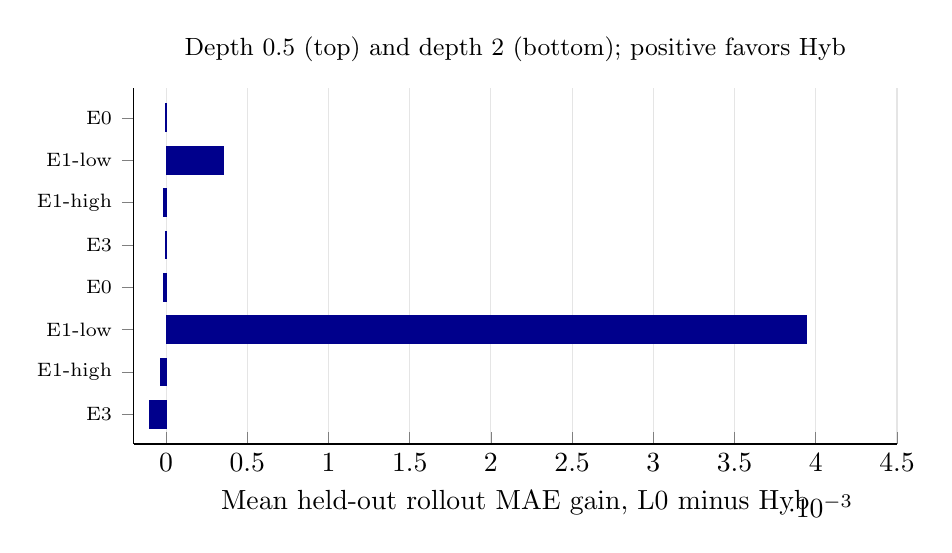
\begin{tikzpicture}
\begin{axis}[
  xbar, width=0.93\textwidth, height=6.1cm,
  xmin=-0.0002, xmax=0.0045,
  xlabel={Mean held-out rollout MAE gain, L0 minus Hyb},
  symbolic y coords={C1,C2,C3,C4,C5,C6,C7,C8}, ytick=data,
  yticklabels={E0, E1-low, E1-high, E3, E0, E1-low, E1-high, E3},
  yticklabel style={font=\scriptsize},
  y dir=reverse, xmajorgrids=true, grid style={gray!20},
  axis x line*=bottom, axis y line*=left,
  title style={font=\small}, title={Depth 0.5 (top) and depth 2 (bottom); positive favors Hyb}
]
\addplot[fill=blue!55!black,draw=blue!55!black] coordinates {
  (-0.000002,C1) (0.000354,C2) (-0.000014,C3) (-0.000003,C4)
  (-0.000017,C5) (0.003943,C6) (-0.000033,C7) (-0.000101,C8)
};
\end{axis}
\end{tikzpicture}
\caption{Cell-averaged recursive price-error MAE gain by operating condition and depth. Each bar averages four held-out shock sizes; cell-level contrasts are descriptive and do not have separate confidence intervals. The underlying values are exported in \code{figures/data/hybrid\_depth\_condition.csv}.}
\label{fig:hybrid-cell-gains}
\end{figure}

The hybrid map’s mean gain should not be read in isolation: nearly all its gain comes from one low-capacity/depth combination, while flow-pressure prediction does not improve. The next modeling step is to represent capacity-binding and LP-withdrawal transitions explicitly and test them with another frozen protocol, rather than to add more free polynomial terms. The map comparison is a predictive surrogate diagnostic. It does not establish a Lyapunov function, local stability for the piecewise map, or stochastic stability for the complete simulator.

\section{Trajectories by depth}

Figure~\ref{fig:prof} compares E1-high and E3 with $\kappa=0.5$. At the lowest depth, E3 starts from the same initial excess and is corrected more slowly. A compatible explanation is that withdrawal lowers both depth and the arbitrage cap $c\,x$; these mechanisms are coupled in the current design. With $\kappa=1$ and $2$ the two trajectories are almost identical. The sustained return occurs on average at tick $7.8$ for E3 with $\kappa=0.5$ against $2.8$ for E1-high, whereas with $\kappa=1$ and $2$ the differences are $0.1$ ticks or less.

\begin{figure}[htbp]
\centering
\begin{tikzpicture}
\begin{axis}[width=0.9\textwidth,height=6.2cm,xlabel={Tick},ylabel={Mean $|d_t|$},grid=major,legend style={font=\scriptsize},xmin=0,xmax=20,ymin=0]
\addplot[thick,blue!70!black] table[col sep=comma,x=tick,y=mean_abs_excess,restrict expr to domain={\thisrow{series_id}}{31:31}] {\datadir/trajectories.csv};
\addplot[thick,dashed,green!50!black] table[col sep=comma,x=tick,y=mean_abs_excess,restrict expr to domain={\thisrow{series_id}}{41:41}] {\datadir/trajectories.csv};
\legend{E1-high,E3}
\end{axis}
\end{tikzpicture}
\caption{Mean excess error with $\kappa=0.5$: static high arbitrage (E1-high) and with adaptive withdrawal (E3).}
\label{fig:prof}
\end{figure}

\section{Engineering sensitivity: recovery and order scale}
\label{sec:engineering-sensitivity}

A supplementary analysis (analysis 0.6.0, run \code{\EngineeringRunID}) used 300 new seeds (2000--2299), three order-flow variants and the 15 depth/shock/condition cells of the held-out grid: 40\,500 paths, 20 abstract ticks each. It is a descriptive and exploratory sensitivity analysis, not an inferential test. Recovery means the first observed pair of consecutive ticks inside the band; a later departure is counted separately. Deadlines are ticks, not elapsed time.

With the original fixed absolute order sizes, adaptive E3 recovered at least once in 97.4\,\% of paths, yet only 81.9\,\% ended in-band. Of paths that recovered, 31.2\,\% later departed. At depth 0.5, only 45.8\,\% ended in-band and 98.8\,\% of recovered paths later departed. Thus a first sustained return is not equivalent to persistent tracking in this model. These equally weighted design averages carry no multiplicity-adjusted population claim.

The depth-specific adaptive-minus-static maximum-response contrast changes with order definition (table~\ref{tab:engineering-sensitivity}). Holding absolute orders fixed produced an effect at depth 0.5, while scaling the noise and trend orders with initial reserves made the contrast effectively zero at all three depths. Disabling the panic sale reduced the shallow-depth contrast but did not eliminate it. This isolates an important model boundary: depth alone does not determine the result; order size relative to reserves and the reaction rule matter.

\begin{table}[htbp]
\centering
\caption{Supplementary paired adaptive-minus-static maximum response by depth (300 new seeds). Approximate 95\,\% intervals are unadjusted.}
\label{tab:engineering-sensitivity}
\small
\begin{tabular}{@{}lrrr@{}}
\toprule
Order-flow variant & Depth 0.5 & Depth 1 & Depth 2 \\
\midrule
Fixed absolute orders & 0.03458 [0.03225, 0.03690] & 0.00000 & 0.00000 \\
Orders proportional to initial reserves & 0.00000 & 0.00000 & 0.00000 \\
Fixed orders, panic disabled & 0.01471 [0.01364, 0.01577] & 0.00000 & 0.00000 \\
\bottomrule
\end{tabular}
\end{table}

At depth 0.5 under fixed absolute orders, adaptive E3 ended in-band in 45.8\,\% of paths; with proportional orders it ended in-band in 100\,\%. These variants still share the same stylized representative-agent model and are not empirical comparisons. The complete cell summaries, paired contrasts, configuration and hashes are exported under \code{figures/engineering/}.

\section{Summary of the results}

\begin{itemize}
  \item \textbf{Analytical arbitrage benchmark:} an isolated pool with capacity $c$ reduces out-of-band log error by at most $2\log(1+c)$ per tick. At $c=0.005$ the ideal correction time for the tested large shock is the full 20-tick horizon; the sign of the active-arbitrage effect follows from the specified rule.
  \item \textbf{Withdrawal sensitivity:} the existing trigger fires in every adaptive-condition run. The legacy pre-shock displacement statistic is sensitive to the depth and order convention; its shallow-depth effect disappears when orders scale with reserves. It does not establish general liquidity amplification.
  \item \textbf{Recovery persistence:} 31.2\,\% of paths that returned to the band later left it, and at depth factor $0.5$ the share was 98.8\,\%. First return and sustained tracking are distinct outcomes in this simulator.
  \item \textbf{Reduced models:} the two-state map improves on persistence in some conditions but does not beat scalar AR(1). The band-aware map's approximately 1.7\,\% replay-error gain is concentrated in one condition and uses the realized future CEX path.
\end{itemize}
